\documentclass[border=4pt]{standalone}
\usepackage[T1]{fontenc}
\usepackage{helvet}
\renewcommand{\familydefault}{\sfdefault}
\usepackage{graphicx}
\usepackage{caption}
\usepackage{amsmath}
\captionsetup{font={sf,footnotesize},labelfont={sf,bf,footnotesize},justification=justified,singlelinecheck=false}
\begin{document}
\setcounter{figure}{6}
\begin{minipage}{7.20in}
\centering
\begin{figure}[htbp]
    \centering
    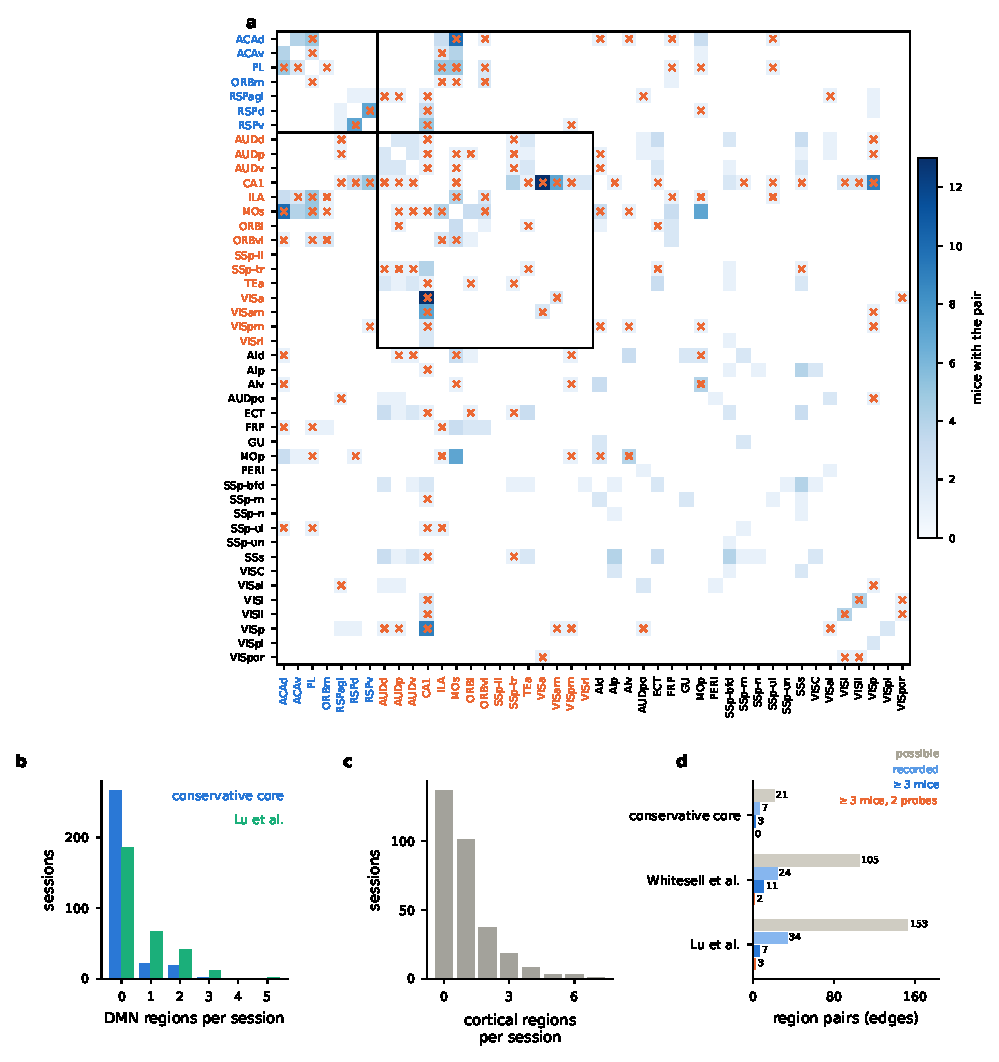
\includegraphics[width=\linewidth]{fig7_coverage_panels.pdf}
    \caption{\textbf{a} Core DMN region pairs with grey-screen co-fluctuation data: number of mice with both regions recorded ($\geq$5 neurons each) in the same session with $\geq$120 still 1 s bins; in brackets, mice in which the pair is recorded on two different probes; grey, never recorded. Boxes: frontal core (ACA, PL, ORBm) and RSP. No frontal-RSP pair is ever recorded. \textbf{b} Number of core regions recorded per session, out of 308 sessions with region signals. \textbf{c} Number of cortical regions recorded per session; most sessions record none or one. \textbf{d} Core region pairs: possible, recorded at least once, recorded in $\geq$3 mice and recorded on two different probes in $\geq$3 mice. The frontal-to-RSP edge at the centre of every DMN map is recorded in 0 sessions.}
    \label{fig:grey_coverage}
\end{figure}
\end{minipage}
\end{document}
